\documentclass[12pt,3p]{article}
\usepackage[utf8]{inputenc}
\usepackage[english]{babel}
\usepackage[margin=0.5in]{geometry}
\usepackage{amsmath}
\usepackage{mathtools}
\usepackage{enumitem}
\usepackage{physics}
\usepackage[round,numbers]{natbib}
\usepackage[colorlinks = false]{hyperref}
\usepackage{tcolorbox}
\usepackage{xcolor}
\usepackage{amsmath}
\usepackage{cleveref} % Refer to range of equations
\usepackage{stmaryrd} % For double brackets for M jump
%This line makes .eps figures into .pdf
\usepackage{epstopdf}
\usepackage{bm}

\setcounter{tocdepth}{4} 
\setcounter{secnumdepth}{4}

\numberwithin{equation}{section}
\begin{document}

\title{Poroelasticity formulation with surface effects \\
	\Large{Updated: \today} \vspace{-2ex}}
\author{Ida Ang}
\date{\vspace{-5ex}}
\maketitle

\tableofcontents
\newpage

\section{Definitions}
\vspace{-2ex}

$f_i$: nominal body force per unit volume \\
$T_i$: nominal traction on surface [force per area] \\
$\sigma_{ij}$: true stress $\rightarrow$ $S_{iJ}$: nominal stress 
\begin{equation*}
\bigg[ \frac{\text{Force}}{\text{Area}} \bigg] 
\end{equation*}
U: free energy of the gel \\
	\indent 
	$U_e$: elastic energy from stretching a polymer network \\
	\indent
	$U_m$: energy of mixing the solvent with polymer chains
\begin{equation*}
\bigg[ \frac{\text{Force}}{\text{Area}} \bigg] 
\end{equation*}
N: number of polymer chains per unit volume in the reference state 
\begin{equation*}
\bigg[ \frac{\text{Number of polymer chains}}{\text{Volume}} \bigg]
\end{equation*}
$k_B$: Boltzmann's Constant
\begin{equation*}
\bigg[ \frac{\text{Energy}}{\text{Temperature}} \bigg] = \bigg[ \frac{\text{Force} \times \text{Length}}{\text{Temperature}} \bigg] 
\end{equation*}
T: [Temperature] \\
K: Shear Modulus (Same units as $N k_B T$)
\begin{equation*}
\bigg[\text{Number of Polymer Chains} \times \frac{\text{Force}}{\text{Area}} \bigg] 
\end{equation*}
$\chi$: Flory-Huggins parameter for the enthalpy of mixing [dimensionless] \\
\textbf{F}: Deformation gradient [dimensionless] \\
C(\textbf{X}): Nominal concentration of solvent per unit volume in reference state \\
c(\textbf{X},t): True concentration of solvent per unit volume in current state \\
\begin{equation*}
\bigg[ \frac{\text{Concentration of Solvent}}{\text{Volume}} \bigg] 
\end{equation*}
$\Omega$: [Volume] \\
$\mu$(\textbf{X},t): chemical potential of the small molecules 
\begin{equation*}
\bigg[ \frac{\text{Energy}}{\text{Concentration}} \bigg] = \bigg[ \frac{\text{Force} \times \text{Length}}{\text{Concentration}} \bigg] 
\end{equation*}
dA(\textbf{X}): element of area [Area] $\rightarrow$ dV(\textbf{X}): element of volume [Volume] \\
$N_K (\textbf{X})$: unit vector normal to the interface in the reference state $\rightarrow$ $n_i (\textbf{X}, t)$: current state [Dimensionless] \\
Number of small molecules injected into: \\
	\indent r(\textbf{X},t): a volume element 
	\begin{equation*}
	\bigg[ \frac{\text{Number of small molecules}}{\text{Volume} \times \text{Time}} \bigg] 
	\end{equation*}
	\indent i(\textbf{X},t): an interface element 
	\begin{equation*}
	\bigg[ \frac{\text{Number of small molecules}}{\text{Area} \times \text{Time}} \bigg] 
	\end{equation*}
D: Solvent diffusivity 
\begin{equation*}
\bigg[ \frac{\text{Area}}{\text{Time}} \bigg]
\end{equation*}
$J_K$: nominal flux $\rightarrow j_i(\mathbf{X},t)$: true flux 
\begin{equation*}
\bigg[ \frac{\text{Number of Small Molecules}}{\text{Time} \times \text{Area}} \bigg] 
\end{equation*}
$M_{KL}$: Nominal mobility tensor
\begin{equation*}
\bigg[ \frac{\text{Number of Small Molecules}}{\text{Time} \times \text{Volume}} \bigg]
\end{equation*}

\newpage

%========================================================================
%========================================================================
%========================================================================
\section{Formulation}
\vspace{-2ex}
This document contains some extra derivations related to my first author paper `Effect of elastocapillarity on the swelling kinetics of hydrogels.' Variables are not defined as carefully as in the paper, as this is meant to be a supplemental reference to the paper. 

%% ==================================================================
%% ==================================================================
\subsection{Kinematics}
\vspace{-1ex}
The displacement, $\mathbf{u}$, is the difference between points in the reference and points in the current configuration, which are denoted by $\mathbf{X}$ and $\mathbf{x}$ respectively. 
\begin{equation}\label{EqDisp}
\mathbf{u} = \mathbf{X} - \mathbf{x}
\end{equation}
By taking the gradient in the reference configuration of Eq. \ref{EqDisp}.
\begin{align*}
\pdv{\mathbf{u}}{\mathbf{X}} 
	&= \pdv{\mathbf{X}}{\mathbf{X}} - \pdv{\mathbf{x}}{\mathbf{X}} \\
\nabla \mathbf{u}
	&= \mathbf{I} - \mathbf{F}
\end{align*}
Therefore, the deformation gradient $\mathbf{F}$ maps the reference configuration to the current configuration. 
\begin{equation}\label{EqDefGrad}
\mathbf{F} = \pdv{\mathbf{x}}{\mathbf{X}} \rightarrow F_{ij} = \pdv{x_i}{X_j}
\end{equation}
and the following relationship is given, where $\mathbf{I}$ is the identity tensor. 
\begin{equation}\label{EqDefGrad2}
\mathbf{F} = \mathbf{I} + \nabla \mathbf{u} 
\end{equation}
The right Cauchy Green (CG) tensor $\mathbf{C}$ is defined as follows
\begin{equation}\label{EqRightCG}
\mathbf{C} = \mathbf{F}^T \mathbf{F}
\end{equation}
The invariants of the right CG tensor are defined as follows.
\begin{align*}
I_\mathbf{C} &= \tr \mathbf{C} \\
II_\mathbf{C} &= \frac{1}{2} (C_{kk}^2 - C_{ik} C_{ki}) \\
III_\mathbf{C} &= \det \mathbf{C} 
\end{align*}
Therefore, we can characterize the volumetric ratio between the current and reference configuration as, where we identify a relationship. 
\begin{equation}
J = \det \mathbf{F} \rightarrow J^2 = III_\mathbf{C}
\end{equation}
Considering the kinematics of continua with boundaries, the surface deformation gradient can be described as follows.
\begin{subequations}\label{EqDefGradSurf}
\begin{align}
\bar{\mathbf{F}} &= \pdv{x_i}{X_K} \cdot \bar{\mathbf{I}} \\
\bar{\mathbf{F}} &= \mathbf{F} \cdot \bar{\mathbf{I}}
\end{align}
\end{subequations}
where the mixed-variant surface unit tensor in the material configuration is:
\begin{align}\label{EqSurfUnitTensor}
\bar{\mathbf{I}} = \mathbf{I} - \mathbf{N} \otimes \mathbf{N}
\end{align}
Just as how the Jacobian describes the change in volume, the surface Jacobian describes the change in surface area. 
\begin{subequations}\label{EqJBulkSurf}
\begin{align}
J &= \frac{dv}{dV} = \det \mathbf{F} \\
\bar{J} &= \frac{da}{dA} = | \underbrace{\det \mathbf{F} \mathbf{F}^{-T}}_\text{cofactor} \mathbf{N} | 
\end{align}
\end{subequations}
The Nanson operator is used to define the surface jacobian, $\bar{J}$
\begin{align}\label{surfaceJacobian}
\begin{split}
\bar{J} &= | J \mathbf{F}^{-T} \mathbf{N} | \\
\bar{J} &= | \underbrace{\det \mathbf{F} \mathbf{F}^{-T}}_\text{cofactor} \mathbf{N} | 
\end{split}	   
\end{align}


%========================================================================
%========================================================================
\subsection{Strong and Weak Forms}
\vspace{-1ex}
We have two sets of partial differential equations (PDEs) that describe the coupled problem. First is the mechanical equilibrium equation and the other is the mass conservation equation describing the balance of mass entering the volume or surface respectively. The mechanical equilibrium equation is phrased in the referential configuration. 
\begin{subequations}\label{EqMechEqm}
\begin{align}
\bm{\nabla}_{\boldsymbol{X}} \cdot \mathbf{P}+\mathbf{b}_{\mathbf{0}} &= \mathbf{0} \quad \text { in } \quad V\\
\mathbf{P} \cdot \mathbf{N}-\overline{\boldsymbol{\nabla}}_{\boldsymbol{X}} \cdot \overline{\mathbf{P}}&=\check{\mathbf{T}} \quad \text { on } \quad S^{T}\\
\mathbf{u} &= \check{\mathbf{u}} \quad \text { on } \quad S^{u}\\
\llbracket \overline{\mathbf{P}} \cdot \overline{\mathbf{N}} \rrbracket &=0 \quad \text { on } \quad L
\end{align}
\end{subequations}
where we use a check to indicate prescribed quantities, such as prescribed tractions, $\mathbf{\check{T}}$,  and displacements, $\mathbf{\check{u}}$. An addition to the usual traction equation $\mathbf{P} \cdot \mathbf{N} = \mathbf{T}$, is made to take into account surface mechanics. $\bar{\mathbf{N}}$ indicates the binormal vector to the boundary curve, L. The double brackets in Eq.\ref{EqMechEqm}d indicate summation over the two surfaces that intersect on the boundary curve.

The mass conservation equation can be stated as follows: 
\begin{subequations}\label{EqMassCon}
\begin{align}
\dot{C}+\nabla_{X} \cdot \mathbf{J} &=r \quad \text { in } \quad V \\
\mathbf{J} \cdot \mathbf{N} &=-i \quad \text { on } \quad S^{i} \\
\mu &= \check{\mu} \quad \text { on } \quad S^{\mu}
\end{align}
\end{subequations}
Equations \ref{EqMechEqm} and \ref{EqMassCon} are solved together for displacements and chemical potential respectively. Taylor Hood elements are utilized for stability.  

In order to obtain the weak form, rearrange Eq. \ref{EqMechEqm}a, multiply with a test function $\delta \boldsymbol\varphi$, and integrate over the domain of interest.
\begin{align*}
\int (\div \mathbf{P}) \cdot \delta \boldsymbol\varphi dV + \int \mathbf{b_o} \cdot \delta \boldsymbol\varphi dV &= 0 \quad \text{Int by Parts} \\
\int \div (\mathbf{P^T} \cdot \delta \boldsymbol\varphi) dV - \int \mathbf{P} \cdot \grad \delta \boldsymbol\varphi dV+ \int \mathbf{b_o} \cdot \delta \varphi dV &= 0 \quad \text{Divergence} \\
\int (\mathbf{P} \cdot \mathbf{N}) \cdot \delta \boldsymbol\varphi dS - \int \mathbf{P} \cdot \grad \delta \boldsymbol\varphi dV+ \int \mathbf{b_o} \cdot \delta \boldsymbol\varphi dV &= 0 \quad \\
\int (\bar{\div} \mathbf{\bar{P}}) \cdot \delta \boldsymbol\varphi dS + \int \mathbf{\bar{b}_o} \cdot \delta \boldsymbol\varphi dS - \int \mathbf{P} \cdot \grad \delta \boldsymbol\varphi dV+ \int \mathbf{b_o} \cdot \delta \boldsymbol\varphi dV &= 0 \quad \text{Int by Parts}\\
\int \bar{\div} (\mathbf{\bar{P}}^T \cdot \delta \boldsymbol\varphi) dS - \int \mathbf{\bar{P}} \cdot \bar{\nabla} \delta \boldsymbol\varphi dS + \int \mathbf{\bar{b}_o} \cdot \delta \boldsymbol\varphi dS - \int \mathbf{P} \cdot \grad \delta \boldsymbol\varphi dV+ \int \mathbf{b_o} \cdot \delta \boldsymbol\varphi dV &= 0 \quad \text{Divergence} \\
\int (\mathbf{\bar{P}} \cdot \mathbf{M}) \cdot \delta \boldsymbol\varphi dL - \int \mathbf{\bar{P}} \cdot \bar{\nabla} \delta \boldsymbol\varphi dS + \int \mathbf{\bar{b}_o} \cdot \delta \boldsymbol\varphi dS - \int \mathbf{P} \cdot \grad \delta \boldsymbol\varphi dV+ \int \mathbf{b_o} \cdot \delta \boldsymbol\varphi dV &= 0 \\
- \int \mathbf{\bar{P}} \cdot \bar{\nabla} \delta \boldsymbol\varphi dS + \int \mathbf{\bar{b}_o} \cdot \delta \boldsymbol\varphi dS - \int \mathbf{P} \cdot \grad \delta \boldsymbol\varphi dV+ \int \mathbf{b_o} \cdot \delta \boldsymbol\varphi dV &= 0 
\end{align*}
Rearrange 
\begin{equation}\label{EqMechWeakForm}
\int \mathbf{\bar{P}} \cdot \bar{\nabla} \delta \boldsymbol\varphi \, dS 
+ \int \mathbf{P} \cdot \grad \delta \boldsymbol\varphi \,dV 
= \int \mathbf{\bar{b}_o} \cdot \delta \boldsymbol\varphi \,dS 
+ \int \mathbf{b_o} \cdot \delta \boldsymbol\varphi \, dV
\end{equation}
Multiply Eq. \ref{EqMassCon} with a scalar test function $\mu$ and follow the same steps as above: 
\begin{align*}
\int {\dot{C}} \delta \mu dV + \int ( \div \mathbf{J}) \delta \mu dV &= \int r \delta \mu dV \quad \text{Int by Parts} \\ 
\int {\dot{C}} \delta \mu dV + \int \div (\mathbf{J}^T \delta \mu) dV - \int \mathbf{J} \cdot \grad \delta \mu dV &= \int r \delta \mu dV \quad \text{Divergence} \\
 \int {\dot{C}} \delta \mu dV + \int (\mathbf{J} \cdot \mathbf{N}) \delta \mu dV - \int \mathbf{J} \cdot \grad \delta \mu dV &= \int r \delta \mu dV \\
 \int {\dot{C}} \delta \mu dV - \int i \delta \mu dS - \int \mathbf{J} \cdot \grad \delta \mu dV &= \int r \delta \mu dV 
\end{align*}
Therefore we obtain the following weak form for the mass conservation equation.
\begin{equation}\label{EqMassConWeakForm}
 \int {\dot{C}} \delta \mu \, dV - \int \mathbf{J} \cdot \grad \delta \mu \, dV = \int r \delta \mu \, dV + \int i \delta \mu \, dS 
\end{equation}

%========================================================================
%========================================================================
\subsection{Time Integration}
\vspace{-1ex}
The weak forms are as followed: 
\begin{align*}
\int \mathbf{\bar{P}} \cdot \bar{\nabla} \delta \boldsymbol\varphi dS  &= \int \mathbf{\bar{b}_o} \cdot \delta \boldsymbol\varphi dS \\
\int \mathbf{P} \cdot \grad \delta \boldsymbol\varphi dV &= \int \mathbf{b_o} \cdot \delta \boldsymbol\varphi dV \\
\int \pdv{C}{t} \delta \mu dV - \int \mathbf{J} \cdot \grad \delta \mu dV &= \int r \delta \mu dV + \int i \delta \mu dS 
\end{align*}
The first two weak forms are not time-dependent (all in current time step) \\ \\
Backward Euler Scheme on the second weak form where \textbf{superscript t indicates previous time step} and no superscript indicates current time step
\begin{align*}
\int \frac{C - C^t}{\Delta t} \delta \mu dV - \int \mathbf{J} \cdot \frac{\delta \mu}{\delta X} dV - \int i \delta \mu dS - \int r \delta \mu dV &= 0 \\
\int (C - C^t) \delta \mu dV - \int \mathbf{J} \cdot \frac{\delta \mu}{\delta X} \Delta t dV - \int i \delta \mu \Delta t dS - \int r \delta \mu \Delta t dV &= 0 
\end{align*}


%========================================================================
%========================================================================
\subsection{Thermodynamic Theory}
\vspace{-1ex}
Surfaces of bodies and interfaces between bodies exhibit different properties from the bulk. These effects can be modeled in terms of surface tension or an added term to the total potential energy, denoted by a bar 
\begin{align*} 
\text{Bulk}&: U = U_e + U_m - \mu C \\
\text{Surface}&:\bar{U} = u_e
\end{align*}
Here, we assume that the surface only has an elastic component. The free energy density of the system changes at the rate: 
\begin{align*}
\delta U (\mathbf{F}, \mu) &= \pdv{U (\mathbf{F}, \mu)}{\mathbf{F}} \delta \mathbf{F}+ \pdv{U (\mathbf{F}, \mu)}{\mu} \delta \mu \\
\delta \bar{U} (\mathbf{\bar{F}}) &=  \pdv{u_e (\mathbf{\bar{F}})}{\mathbf{\bar{F}}} \delta \mathbf{\bar{F}}
\end{align*}
Taking in the sum 
\begin{align*}
 \frac{\delta G_{bulk}}{\delta t} &= \int \frac{\delta U}{\delta t} dV  - \int \mathbf{b_o} \frac{\delta \mathbf{x}}{\delta t} dV - \int \mu r dV - \int \mu i dS \\
\frac{\delta G_{surf}}{\delta t} &= \int \frac{\delta \bar{U}}{\delta t} dS - \int_{S} \check{\mathbf{T}} \frac{\delta \overline{\mathbf{x}}}{\delta t} d S 
\end{align*}
Together the gel and field of weights and pumps form a thermodynamic system
\begin{align*}
\frac{\delta G}{\delta t} &= \frac{\delta G_{bulk}}{\delta t} + \frac{\delta G_{surf}}{\delta t} \\
\frac{\delta G}{\delta t} &= \int_{V} \frac{\delta U}{\delta t} d V + \int_{S} \frac{\delta \bar{U}}{\delta t} d S - 
\underbrace{\int_{V} \mathbf{b}_{\mathbf{0}} \frac{\delta \mathbf{x}}{\delta t} d V - \int_{S} \check{\mathbf{T}} \frac{\delta \overline{\mathbf{x}}}{\delta t} d S}_\text{Rate of mechanical work}
- \underbrace{\int_{V} \mu r d V-\int_{S} \mu i d S}_\text{Rate of chemical work} 
\end{align*}
The change in free energy density over time 
\begin{align*}
\pdv{U}{t} &= \pdv{U}{\mathbf{F}} \frac{\delta \mathbf{F}}{\delta t}+ \pdv{U}{\mu} \frac{\delta \mu}{\delta t} + \frac{\delta (\mu C)}{\delta t} \\
\pdv{u_e}{t} &= \pdv{u_e}{\mathbf{\bar{F}}} \frac{\delta \mathbf{\bar{F}}}{\delta t}
\end{align*}
Rephrase the two weak forms where $\delta u$ is equivalent to $\delta \mathbf{x} / \delta t$ or $\delta \mathbf{\bar{x}} / \delta t $
\begin{align*}
\int \mathbf{\bar{P}} \cdot \bar{\nabla} \frac{\delta \mathbf{\bar{x}}}{\delta t} dS  &= \int \mathbf{\bar{b}_o} \cdot \frac{\delta \mathbf{\bar{x}}}{\delta t} dS 
\quad \rightarrow \quad 
\int \mathbf{\bar{P}} \cdot \frac{\delta \mathbf{\bar{F}}}{\delta t} dS = \int \mathbf{\bar{b}_o} \cdot \frac{\delta \mathbf{\bar{x}}}{\delta t} dS \\
\int \mathbf{P} \cdot \grad \frac{\delta \mathbf{x}}{\delta t} dV &= \int \mathbf{b_o} \cdot \frac{\delta \mathbf{x}}{\delta t} dV 
\quad \rightarrow \quad 
\int \mathbf{P} \cdot \frac{\delta \mathbf{F}}{\delta t} dV = \int \mathbf{b_o} \cdot \frac{\delta \mathbf{x}}{\delta t} dV
\end{align*}
Rewrite the weak form from $\delta \mu$ is $\mu$
\begin{align*}
\int \pdv{C}{t}  \mu dV - \int r \mu dV - \int i \mu dS = \int \mathbf{J} \cdot \grad \mu dV
\end{align*}
Bulk 
\begin{align*}
 \frac{\delta G_{bulk}}{\delta t} &= \int \frac{\delta U}{\delta t} dV  - \int \mathbf{b_o} \frac{\delta \mathbf{x}}{\delta t} dV - \int \mu r dV - \int \mu i dS \\
 	&= \int \pdv{U}{\mathbf{F}} \frac{\delta \mathbf{F}}{\delta t} dV + \int \pdv{U}{\mu} \frac{\delta \mu}{\delta t} dV + \int \frac{\delta (\mu C)}{\delta t} dV - \int \mathbf{b_o} \frac{\delta \mathbf{x}}{\delta t} dV - \int \mu r dV - \int \mu i dS \\
	 &= \int \pdv{U}{\mathbf{F}} \frac{\delta \mathbf{F}}{\delta t} dV + \int \pdv{U}{\mu} \frac{\delta \mu}{\delta t} dV + \int \frac{\delta \mu}{\delta t} C dV + \int \mu \frac{\delta C}{\delta t} dV- \int \mathbf{P} \cdot \frac{\delta \mathbf{F}}{\delta t} dV - \int \mu r dV - \int \mu i dS \\
	 &= \int \bigg( \pdv{U}{\mathbf{F}} - \mathbf{P} \bigg) \frac{\delta \mathbf{F}}{\delta t} dV + \int \bigg( \pdv{U}{\mu} + C \bigg) \frac{\delta \mu}{\delta t} dV + \int \mu \frac{\delta C}{\delta t} dV - \int \mu r dV - \int \mu i dS \\
 \frac{\delta G_{bulk}}{\delta t} &= \int \bigg( \pdv{U}{\mathbf{F}} - \mathbf{P} \bigg) \frac{\delta \mathbf{F}}{\delta t} dV + \int \bigg( \pdv{U}{\mu} + C \bigg) \frac{\delta \mu}{\delta t} dV + \int \mathbf{J} \cdot \grad \mu dV
\end{align*}
Surface
\begin{align*}
\frac{\delta G_{surf}}{\delta t} &= \int \frac{\delta \bar{U}}{\delta t} dS - \int \mathbf{\bar{b}_o} \frac{\delta \bar{x}}{\delta t} dS \\
	&= \int \pdv{\bar{U}}{\mathbf{\bar{F}}} \frac{\delta \mathbf{\bar{F}}}{\delta t} dS - \int \mathbf{\bar{b}_o} \frac{\delta \bar{x}}{\delta t} dS \\
	&= \int \pdv{\bar{U}}{\mathbf{\bar{F}}} \frac{\delta \mathbf{\bar{F}}}{\delta t} dS - \int \mathbf{\bar{P}} \cdot \frac{\delta \mathbf{\bar{F}}}{\delta t} dS \\
\frac{\delta G_{surf}}{\delta t} &= \int \bigg( \pdv{\bar{U}}{\mathbf{\bar{F}}} - \mathbf{\bar{P}} \bigg)  \frac{\delta \mathbf{\bar{F}}}{\delta t} dS 
\end{align*}
Therefore 
\begin{align}\label{EqFreeEnergyRate}
\frac{\delta G}{\delta t} = \int \bigg( \pdv{U}{\mathbf{F}} - \mathbf{P} \bigg) \frac{\delta \mathbf{F}}{\delta t} dV + \int \bigg( \pdv{\bar{U}}{\mathbf{\bar{F}}} - \mathbf{\bar{P}} \bigg)  \frac{\delta \mathbf{\bar{F}}}{\delta t} dS + \int \bigg( \pdv{U}{\mu} + C \bigg) \frac{\delta \mu}{\delta t} dV + \int \mathbf{J} \cdot \pdv{\mu}{X} dV
\end{align}
The second law of thermodynamics dictates that the free energy of the system should never increase: 
\begin{align}\label{EqSecondLawTherm}
\frac{\delta G}{\delta t} \leq 0 
\end{align}
This leads to the following expressions for the Piola Kirchoff stresses and the concentration: 
\begin{subequations}\ref{EqState}
\begin{align}
\mathbf{P} &= \pdv{U}{\mathbf{F}} \\
\mathbf{\bar{P}} &= \pdv{\bar{U}}{\mathbf{\bar{F}}} \\
C &= -\pdv{U}{\mu}
\end{align}
\end{subequations}

%========================================================================
%========================================================================
\subsection{Kinetic Law}
\vspace{-1ex}
We enforce the negative definite structure of the last integrand in Eq. \ref{EqFreeEnergyRate} by adopting a kinetic law
\begin{equation}\label{EqKinLaw}
\mathbf{J} = - \mathbf{M} \cdot \pdv{\mu}{X} = - \mathbf{M} \cdot \grad \mu
\end{equation}
We can obtain the structure of the mobility tensor with the following derivation. The flux relates to the gradient of the chemical potential
\begin{equation}\label{25}
\mathbf{j} = - \frac{cD}{kT} \pdv{\mu}{x}
\end{equation}
The true concentration relates to the nominal concentration as: 
\begin{equation}\label{26}
c = \frac{C}{\det \mathbf{F}}
\end{equation}
Recall an identity 
\begin{equation}\label{identity2}
\det (\mathbf{F}) \mathbf{N} dA = \mathbf{F} \mathbf{n} da \rightarrow \frac{\mathbf{N} dA}{\mathbf{n} da} = \frac{\mathbf{F}}{\det \mathbf{F}}
\end{equation}
The number of molecules crossing the material element per unit time can be written:
\begin{equation}\label{27}
\mathbf{j} \cdot \mathbf{n} da = \mathbf{J} \cdot \mathbf{N} dA
\end{equation}
Consequently, relate the true flux to the nominal flux.
\begin{align*}
\mathbf{j} &= \mathbf{J} \cdot \frac{\mathbf{N} dA}{\mathbf{n} da} \quad \text{substitute Eq. \ref{identity2}}\\
    &= \mathbf{J} \frac{\mathbf{F}}{\det \mathbf{F}} \quad \text{substitute Eq. \ref{kinLaw}} \\
    &= -\mathbf{M} \cdot \pdv{\mu}{X} \frac{\mathbf{F}}{\det \mathbf{F}} \quad \text{use chain rule} \\
    &= - \mathbf{M} \pdv{\mu}{x} \pdv{x}{X} \frac{\mathbf{F}}{\det \mathbf{F}} \quad \text{use Eq. \ref{25}} \\
- \frac{cD}{k_B T} \pdv{\mu}{x} &= - \mathbf{M} \pdv{\mu}{x} \pdv{x}{X} \cdot \pdv{x}{X} \frac{1}{\det \mathbf{F}} \\
- \frac{cD}{k_B T} \det \mathbf{F} &= - \mathbf{M} \pdv{x}{X} \cdot \pdv{x}{X} \\
- \frac{CD}{k_B T} &= - \mathbf{M} \pdv{x}{X} \cdot \pdv{x}{X} \\
\end{align*}
Rearrange in terms of $M_{KL}$, use Eq. \ref{26} and invoke incompressibility
\begin{equation}\label{EqMobilityTensor}
\mathbf{M} = \frac{CD}{k_B T} \mathbf{F}^{-1} \mathbf{F}^{-T} 
\end{equation}

%========================================================================
%========================================================================
\subsection{Strain Energy Density}
\vspace{-1ex}
The constituents of the hydrogel are assumed to be incompressible: 
\begin{equation}\label{incompressible}
\det \mathbf{F} = 1 + \Omega C 
\end{equation}
Free energy due to stretching (Flory, 1953)
\begin{align}\label{Stretch}
\begin{split}
U_e (\boldsymbol{F}) &=  \frac{1}{2} N k_B T \big[ \tr \mathbf{C} - 3 - 2 \log (\det \mathbf{F}) \big] 
\end{split}
\end{align}
Flory-Huggins (Flory, 1942; Huggins, 1941) model for the energy of mixing 
\begin{align}\label{Mix}
\begin{split}
U_m(C) &= - \frac{k_B T}{\Omega} \bigg[ \Omega C \log(\frac{1 + \Omega C}{\Omega C}) + \frac{\chi}{1 + \Omega C} \bigg] \quad \text{Use. Eq. \ref{incompressible}} \\
U_m(C) &= - \frac{k_B T}{\Omega} \bigg[ (\det \mathbf{F} - 1) \log(\frac{\det \mathbf{F}}{\det \mathbf{F} - 1}) + \frac{\chi}{\det \mathbf{F}} \bigg] \quad \text{Use log property}\\
U_m(C) &= \frac{k_B T}{\Omega} \bigg[ (\det \mathbf{F} - 1) \log (\frac{\det \mathbf{F} - 1}{\det \mathbf{F}}) - \frac{\chi}{\det \mathbf{F}} \bigg] 
\end{split}
\end{align}
Total strain energy in terms of the deformation gradient: 
\begin{align*}
U (\mathbf{F}, \mu) &= \frac{1}{2} N k_B T \big[ \tr \mathbf{C} - 3 - 2 \log (\det \mathbf{F}) \big] + \frac{k_B T}{\Omega} \bigg[ (\det \mathbf{F} - 1) \log (\frac{\det \mathbf{F} - 1}{\det \mathbf{F}}) - \frac{\chi}{\det \mathbf{F}} \bigg] - \mu \big(\frac{\det \mathbf{F} - 1}{\Omega} \big)
\end{align*}
We can describe the boundary potentials in two separate assumptions. The first assumes a fluid-like assumption for a surface tension boundary potential. 
\begin{align}\label{EqSTPotEnergy}
\bar{U} (\mathbf{\bar{F}}) = \gamma \bar{J}
\end{align}
The other assumes surface elasticity
\begin{align}\label{EqNhPotEnergy}
\bar{U} (\mathbf{\bar{F}}) = \frac{\bar{\lambda}}{2} \log^2 \bar{J} + \frac{\bar{\mu}}{2} (\mathbf{\bar{F}} : \mathbf{\bar{F}} - 2 - 2 \log \bar{J})
\end{align}

\subsubsection{Expressions for 1st Piola-Kirchoff Stress and Concentration}
\vspace{-1ex}
The 1st PK stress and the concentration of the solvent can be obtained from the free energy density: 
\begin{align*}
\mathbf{P} 
	&= \pdv{U}{\mathbf{F}} \\
\mathbf{P} 
	&=  2 \mathbf{F} \pdv{{U}}{I_\mathbf{C}} \pdv{I_\mathbf{C}}{\mathbf{C}} 
	+ \pdv{U}{J} \pdv{J}{\mathbf{F}} 
\end{align*}
First Term:
\begin{align*}
\pdv{U}{I_\mathbf{C}} &= \pdv{U}{\tr \mathbf{C}} = \frac{1}{2} N k_B T 
\end{align*}
Second Term:
\begin{align*}
\pdv{I_\mathbf{C}}{\mathbf{C}} &= \pdv{\tr \mathbf{C}}{\mathbf{C}} \\
\pdv{I_\mathbf{C}}{\mathbf{C}} &= \mathbf{I}
\end{align*}
Third Term:
\begin{align*}
\pdv{U}{J} 
	&= \pdv{}{J} \bigg[ \frac{1}{2} N k_B T \big[\tr \mathbf{C} - 3 - 2 \log J \big] + \frac{k_B T}{\Omega} \big[ (J - 1) \log \big( \frac{J - 1}{J} \big) - \frac{\chi}{J} \big] - \mu \big(\frac{J - 1}{\Omega} \big) \bigg] \\
	&= \frac{1}{2} N k_B T \bigg(-2 \pdv{\log J}{J} \bigg) 
	+ \frac{k_B T}{\Omega} \bigg[ \frac{1}{\det \mathbf{F}} 
	+ \log \bigg( \frac{\det \mathbf{F} - 1}{J} \bigg) 
	+ \frac{\chi}{(J)^2} \bigg] 
	- \frac{\mu}{\Omega} \bigg( \pdv{(J-1)}{J} \bigg)\\
	&= - N k_B T \frac{1}{J} 
	+ \frac{k_B T}{\Omega} \bigg[ \frac{1}{J} + \log \bigg( \frac{(J - 1)}{J} \bigg) + \frac{\chi}{J^2} \bigg] 
	- \frac{\mu}{\Omega} \\
	&= N k_B T \bigg\{- \frac{1}{J} 
	+ \frac{1}{N \Omega} \bigg[ \frac{1}{J} + \log \bigg( \frac{J - 1}{J} \bigg) + \frac{\chi}{J^2} \bigg] - \frac{\mu}{N \Omega k_B T} \bigg\} \\
\pdv{U}{J} 
	&= N k_B T \bigg\{- \frac{1}{J} + \frac{1}{N \Omega} \bigg[ \frac{1}{J} + \log \bigg( \frac{J - 1}{J} \bigg) + \frac{\chi}{J^2} - \frac{\mu}{k_B T} \bigg] \bigg\} 
\end{align*}
Fourth Term: 
\begin{align*}
\pdv{J}{F_{iJ}} &= \pdv{\det \mathbf{F}}{F_{iJ}} \quad \text{where } \pdv{\det \mathbf{F}}{F} = (\det \mathbf{F}) \mathbf{F}^{-T} \\
			&= \det \mathbf{F} F_{iJ}^{-T}
\end{align*}
Substituting in each term,
\begin{align*}
\mathbf{P} 
	&=  2 \mathbf{F} \pdv{{U}}{I_\mathbf{C}} \pdv{I_\mathbf{C}}{\mathbf{C}} 
	+ \pdv{U}{J} \pdv{J}{\mathbf{F}} \\
	&= N k_B T \mathbf{F} \cdot \mathbf{I} + N k_B T \bigg\{- \frac{1}{J} + \frac{1}{N \Omega} \bigg[ \frac{1}{J} + \log \bigg( \frac{J - 1}{J} \bigg) + \frac{\chi}{J^2} - \frac{\mu}{k_B T} \bigg] \bigg\} J \mathbf{F^{-T}} 
\end{align*}
Therefore, we can obtain an explicit expression for the 1st PK stress in Eq. \ref{Eq1PK}.
\begin{equation}\label{Eq1PK}
\mathbf{P} 
	= N k_B T \bigg\{\mathbf{F} - \frac{1}{J} + \frac{1}{N \Omega} \bigg[ \frac{1}{J} + \log \bigg( \frac{J - 1}{J} \bigg) + \frac{\chi}{J^2} - \frac{\mu}{k_B T} \bigg] \bigg\} J \mathbf{F^{-T}}
\end{equation}
The same procedure can be done to obtain the equation for concentration. In this case, it is a simple expression.
\begin{subequations}\label{EqConcentration}
\begin{align}
C (\mathbf{F}, \mu) &= - \frac{\delta U}{\delta \mu} \\
	&= - \bigg( - \frac{\det \mathbf{F} - 1}{\Omega} \bigg) \\
						C (\mathbf{F}, \mu) &= \frac{\det \mathbf{F} - 1}{\Omega}
\end{align}
\end{subequations}


%========================================================================
%========================================================================
%========================================================================
\section{Normalization}
Normalization parameters below:
\begin{align*}
\text{Lengths normalized by thickness (dry)}&: l = \tilde{l} H \\
\text{Surfaces normalized by}&: dA = d \tilde{A} H^2 \\
\text{Volumes normalized by}&: dV = d \tilde{V} H^3 \text{ or } dV = d \tilde{V} \Omega \\ 
\text{Time normalized by}&: t = \tilde{t} \tau \quad \text{where } \tau = \frac{H^2}{D} \\
\text{Chemical Potential normalized by}&: \mu = \tilde{\mu} k_B T \\
\text{Stress normalized by}&: S= \tilde{S} N k_B T \quad \gamma = \tilde{\gamma} N k_B T \\
\text{Concentration normalized by}&: \Omega C = \tilde{C} \rightarrow C = \frac{\tilde{C}}{\Omega} 
\end{align*}
Normalization of nominal stress
\begin{align*}
\mathbf{P} &= N k_B T \bigg \langle \mathbf{F} + \bigg\{- \frac{1}{\det \mathbf{F}} + \frac{1}{N \Omega} \bigg[ \frac{1}{\det \mathbf{F}} + \log \bigg( \frac{\det \mathbf{F} - 1}{\det \mathbf{F}} \bigg) + \frac{\chi}{(\det \mathbf{F})^2} - \frac{\mu}{k_B T} \bigg] \bigg\} \det \mathbf{F} \mathbf{F}^{-T}\bigg \rangle \\
\mathbf{\tilde{P}} N k_B T &= N k_B T \bigg \langle \mathbf{F} + \bigg\{- \frac{1}{\det \mathbf{F}} + \frac{1}{N \Omega} \bigg[ \frac{1}{\det \mathbf{F}} + \log \bigg( \frac{\det \mathbf{F} - 1}{\det \mathbf{F}} \bigg) + \frac{\chi}{(\det \mathbf{F})^2} - \frac{\tilde{\mu} k_B T}{k_B T} \bigg] \bigg\} \det \mathbf{F} \mathbf{F}^{-T}\bigg \rangle \\
\mathbf{\tilde{P}} &= \mathbf{F} + \bigg\{- \frac{1}{\det \mathbf{F}} + \frac{1}{N \Omega} \bigg[ \frac{1}{\det \mathbf{F}} + \log \bigg( \frac{\det \mathbf{F} - 1}{\det \mathbf{F}} \bigg) + \frac{\chi}{(\det \mathbf{F})^2} - \tilde{\mu} \bigg] \bigg\} \det \mathbf{F} \mathbf{F}^{-T} \\
\mathbf{\tilde{P}} &= \mathbf{F} + \bigg\{- \frac{1}{J} + \frac{1}{N \Omega} \bigg[ \frac{1}{J} + \log \bigg( \frac{J - 1}{J} \bigg) + \frac{\chi}{J^2} - \tilde{\mu} \bigg] \bigg\} J \mathbf{F}^{-T}
\end{align*}
Normalization of concentration
\begin{align*}
C &= \frac{(\det \mathbf{F} - 1)}{\Omega} \\
\frac{\tilde{C}}{\Omega} &= \frac{(\det \mathbf{F} - 1)}{\Omega} \\
\tilde{C} &= \det \mathbf{F} - 1 = J - 1
\end{align*}

%========================================================================
%========================================================================
\subsection{Normalization of Weak Forms}
\begin{align*}
\int \mathbf{\bar{P}} \cdot \bar{\nabla} \delta \boldsymbol\varphi dS - \int \mathbf{\bar{b}_o} \cdot \delta \boldsymbol\varphi dS &= 0 \\
\int \mathbf{\tilde{\bar{P}}}H N k_B T \cdot \bar{\nabla} \delta \tilde{\boldsymbol\varphi} d\tilde{S} H^2 - \int \mathbf{\tilde{\bar{b}}_o} N k_B T \cdot \delta \tilde{\boldsymbol\varphi} H d \tilde{S} H^2 &= 0 \\
\int \mathbf{\tilde{\bar{P}}} \Omega N k_B T \cdot \bar{\nabla} \delta \tilde{\boldsymbol\varphi} d\tilde{S} - \int \mathbf{\tilde{\bar{b}}_o} N k_B T \cdot \delta \tilde{\boldsymbol\varphi} d \tilde{S} \Omega &= 0 \\
N \Omega k_B T \bigg[ \int \mathbf{\tilde{\bar{P}}} \cdot \bar{\nabla} \delta \tilde{\boldsymbol\varphi} d\tilde{S} - \int \mathbf{\tilde{\bar{b}}_o} \cdot \delta \tilde{\boldsymbol\varphi} d \tilde{S} \bigg] &= 0 
\end{align*}
\begin{align*}
\int \mathbf{P} \cdot \grad \delta \boldsymbol\varphi dV - \int \mathbf{b_o} \cdot \delta \boldsymbol\varphi dV &= 0\\
\int \mathbf{\tilde{P}} N k_B T \cdot \grad \delta \tilde{\boldsymbol\varphi} d\tilde{V} \Omega - \int \mathbf{\tilde{b}_o} \frac{N k_B T}{H} \cdot \delta \tilde{\boldsymbol\varphi} H d\tilde{V} \Omega &= 0 \\
\int \mathbf{\tilde{P}} N \Omega k_B T \cdot \grad \delta \tilde{\boldsymbol\varphi} d\tilde{V} - \int \mathbf{\tilde{b}_o} N \Omega k_B T \cdot \delta \tilde{\boldsymbol\varphi} d\tilde{V} &= 0 \\
N \Omega k_B T \bigg[ \int \mathbf{\tilde{P}}  \cdot \grad \delta \tilde{\boldsymbol\varphi} d\tilde{V} - \int \mathbf{\tilde{b}_o} \cdot \delta \tilde{\boldsymbol\varphi} d\tilde{V} \bigg] &= 0 
\end{align*}
Combine
\begin{align*}
N \Omega k_B T \bigg[ \int \mathbf{\tilde{\bar{P}}} \cdot \bar{\nabla} \delta \tilde{\boldsymbol\varphi} d\tilde{S} + \int \mathbf{\tilde{P}}  \cdot \grad \delta \tilde{\boldsymbol\varphi} d\tilde{V} - \int \mathbf{\tilde{\bar{b}}_o} \cdot \delta \tilde{\boldsymbol\varphi} d \tilde{S} - \int \mathbf{\tilde{b}_o} \cdot \delta \tilde{\boldsymbol\varphi} d\tilde{V} \bigg] &= 0 \\
\end{align*}
Normalize kinetic law
\begin{align}\label{fluxLawFinNorm}
\begin{split}
\mathbf{J} &= - \frac{CD}{k_B T} \mathbf{F^{-1}} \mathbf{F^{-T}} \pdv{\mu}{X} \\
   		&= - \frac{\tilde{C}}{\Omega} \frac{D}{k_B T} \mathbf{F^{-1}} \mathbf{F^{-T}} \pdv{\mu}{X} \quad \text{where } \tau = H^2/D \\
\mathbf{\tilde{J}} &= - \frac{\tilde{C}}{\Omega} \frac{H^2}{\tau k_B T} \mathbf{F^{-1}} \mathbf{F^{-T}} \pdv{ (\tilde{\mu} k_B T) }{(\tilde{X} H)} \\
\mathbf{\tilde{J}} &= - \frac{\tilde{C}}{\Omega} \frac{H}{\tau} \mathbf{F^{-1}} \mathbf{F^{-T}} \pdv{ \tilde{\mu} }{\tilde{X}} \\
\end{split}
\end{align}
Using the normalized Flux equation, Eq. \ref{fluxLawFinNorm} in the first step 
\begin{align*}
\int (C - C^t) \delta \mu dV - \int \mathbf{J} \cdot \frac{\delta \mu}{\delta X} \Delta t dV - \int i \delta \mu \Delta t dS - \int r \delta \mu \Delta t dV &= 0 \\
\int \frac{(\tilde{C} - \tilde{C}^t)}{\Omega} \delta \tilde{\mu} k_B T d\tilde{V} \Omega - \int \mathbf{\tilde{J}} \cdot \frac{\delta (\tilde{\mu} k_B T)}{\delta \tilde{X} H} \Delta \tilde{t} \tau d \tilde{V} \Omega - \int \frac{\tilde{i}}{H^2 \tau} \delta \tilde{\mu} k_B T \Delta \tilde{t} \tau d\tilde{S} H^2 - \int \frac{\tilde{r}}{\Omega \tau} \delta \tilde{\mu} k_B T \Delta \tilde{t} \tau d \tilde{V} \Omega &= 0 \\
k_B T \int (\tilde{C} - \tilde{C}^t) \delta \tilde{\mu} d\tilde{V} - k_B T\int \mathbf{\tilde{J}} \cdot \frac{\delta \tilde{\mu}}{\delta \tilde{X}} \Delta \tilde{t} \frac{\tau}{H} \Omega d\tilde{V} - k_B T \int \tilde{i} \delta \tilde{\mu} \Delta \tilde{t} d\tilde{S} - k_B T \int \tilde{r} \delta \tilde{\mu}  \Delta \tilde{t} d \tilde{V} &= 0 \\
k_B T \bigg[ \int (\tilde{C} - \tilde{C}^t) \delta \tilde{\mu} d\tilde{V} + \int \frac{\tilde{C}}{\Omega} \frac{H}{\tau} \mathbf{F^{-1}} \mathbf{F^{-T}} \pdv{ \tilde{\mu} }{\tilde{X}} \cdot \frac{\delta \tilde{\mu}}{\delta \tilde{X}} \Delta \tilde{t} \frac{\tau}{H} \Omega d\tilde{V} - \int \tilde{i} \delta \tilde{\mu} \Delta \tilde{t} d\tilde{S} - \int \tilde{r} \delta \tilde{\mu}  \Delta \tilde{t} d \tilde{V} \bigg] &= 0 \\
k_B T \bigg[ \int (\tilde{C} - \tilde{C}^t) \delta \tilde{\mu} d\tilde{V} + \int \tilde{C} \mathbf{F^{-1}} \mathbf{F^{-T}} \pdv{ \tilde{\mu} }{\tilde{X}} \cdot \frac{\delta \tilde{\mu}}{\delta \tilde{X}} \Delta \tilde{t} d\tilde{V} - \int \tilde{i} \delta \tilde{\mu} \Delta \tilde{t} d\tilde{S} - \int \tilde{r} \delta \tilde{\mu}  \Delta \tilde{t} d \tilde{V} \bigg] &= 0 
\end{align*}
Combine two equations and divide by $N \Omega k_B T$, leaving the final normalized weak form 
\begin{align*}
\frac{1}{N \Omega} \bigg[ \int (\tilde{C} - \tilde{C}^t) \delta \tilde{\mu} d\tilde{V} + \int \tilde{C} \mathbf{F^{-1}} \mathbf{F^{-T}} \pdv{ \tilde{\mu} }{\tilde{X}} \cdot \frac{\delta \tilde{\mu}}{\delta \tilde{X}} \Delta \tilde{t} d\tilde{V} - \int \tilde{i} \delta \tilde{\mu} \Delta \tilde{t} d\tilde{S} - \int \tilde{r} \delta \tilde{\mu}  \Delta \tilde{t} d \tilde{V} \bigg] &= 0 \\
\int \mathbf{\tilde{\bar{P}}} \cdot \bar{\nabla} \delta \tilde{\boldsymbol\varphi} d\tilde{S} + \int \mathbf{\tilde{P}}  \cdot \grad \delta \tilde{\boldsymbol\varphi} d\tilde{V} - \int \mathbf{\tilde{\bar{b}}_o} \cdot \delta \tilde{\boldsymbol\varphi} d \tilde{S} - \int \mathbf{\tilde{b}_o} \cdot \delta \tilde{\boldsymbol\varphi} d\tilde{V} &= 0
\end{align*}
where the previous time step is $\tilde{C^t}$

%========================================================================
%========================================================================
%========================================================================
\section{Initial Conditions}
\vspace{-2ex}
%========================================================================
%========================================================================
\subsection{Initial Condition for Chemical Potential without Surface Tension}
\vspace{-1ex}
Initially stress free gel: 
\begin{align*}
\tilde{S} =  F_{iJ} + \bigg\{- \frac{1}{\det \mathbf{F}} + \frac{1}{N \Omega} \bigg[ \frac{1}{\det \mathbf{F}} + \log \bigg( \frac{\det \mathbf{F} - 1}{\det \mathbf{F}} \bigg) + \frac{\chi}{(\det \mathbf{F})^2} - \tilde{\mu} \bigg] \bigg\} \det \mathbf{F} F_{iJ}^{-T} &= 0 \\
		F_{iJ} - F_{iJ}^{-T} + \frac{1}{N \Omega} \bigg[ \frac{1}{\det \mathbf{F}} + \log \bigg( \frac{\det \mathbf{F} - 1}{\det \mathbf{F}} \bigg) + \frac{\chi}{(\det \mathbf{F})^2} - \tilde{\mu} \bigg] \det \mathbf{F} F_{iJ}^{-T} &= 0 \\
		F_{iJ} - F_{iJ}^{-T} + \frac{1}{N \Omega} \bigg[ F_{iJ}^{-T} + \det \mathbf{F} F_{iJ}^{-T} \log \bigg( \frac{\det \mathbf{F} - 1}{\det \mathbf{F}} \bigg) + \frac{\chi}{\det \mathbf{F}} F_{iJ}^{-T}\bigg] &=  \tilde{\mu} \frac{1}{N \Omega} \det \mathbf{F} F_{iJ}^{-T} \\
		 \frac{N \Omega}{\det \mathbf{F} F_{iJ}^{-T}} \bigg( F_{iJ} - F_{iJ}^{-T} \bigg) + \frac{1}{\det \mathbf{F} F_{iJ}^{-T}} \bigg[ F_{iJ}^{-T} + \det \mathbf{F} F_{iJ}^{-T} \log \bigg( \frac{\det \mathbf{F} - 1}{\det \mathbf{F}} \bigg) + \frac{\chi}{\det \mathbf{F}} F_{iJ}^{-T}\bigg] &=  \tilde{\mu} \\
		  \frac{N \Omega}{\det \mathbf{F} F_{iJ}^{-T}} \bigg( F_{iJ} - F_{iJ}^{-T} \bigg) + \frac{1}{\det \mathbf{F}} + \log \bigg( \frac{\det \mathbf{F} - 1}{\det \mathbf{F}} \bigg) + \frac{\chi}{(\det \mathbf{F})^2} &=  \tilde{\mu} \quad \text{where } \det \mathbf{F} = \lambda_o^3 \\
		  N \Omega \frac{\lambda_o}{\lambda_o^3} \bigg( \lambda_o - \frac{1}{\lambda_o} \bigg) + \frac{1}{\lambda_o^3} + \log \bigg( \frac{\lambda_o^3 - 1}{\lambda_o^3} \bigg) + \frac{\chi}{\lambda_o^6} &= \tilde{\mu} 
\end{align*}
This gives the initial normalized chemical potential
\begin{align*}
 \tilde{\mu} = N \Omega \bigg( \frac{1}{\lambda_o} - \frac{1}{\lambda_o^3} \bigg) + \frac{1}{\lambda_o^3} + \log \bigg( \frac{\lambda_o^3 - 1}{\lambda_o^3} \bigg) + \frac{\chi}{\lambda_o^6} 
\end{align*}

%========================================================================
%========================================================================
\subsection{Initial Condition for Chemical Potential with Surface Tension}
\vspace{-1ex}
Paper Reference: \textit{Elastocapillarity: Surface Tension and the Mechanics of Soft Solids} by Style, Jagota, Hui, and Dufresne. \\ \\
The essential idea is a connection between surface stress and bulk stress at the interface. The governing interfacial equation is a condition for static equilibrium. 
\begin{equation*}
\int_{S} \sigma_{1} \cdot \mathbf{n} \mathrm{d} S-\int_{S} \boldsymbol{\sigma}_{2} \cdot \mathbf{n} \mathrm{d} S+\oint_{C} \mathbf{\Upsilon} \cdot \mathbf{b} \mathrm{d} l=0
\end{equation*}
Using the surface divergence theorem, we can obtain the generalization of Laplace's Law
\begin{align*}
\boldsymbol{\sigma} \cdot \mathbf{n} + \tilde{\div} \boldsymbol{\Upsilon} &= 0 \quad \text{Assume surface stress is isotropic} \\
\boldsymbol{\sigma} \cdot \mathbf{n} + \tilde{\div} (\gamma \mathbf{I}) &= 0 \\
\boldsymbol{\sigma} \cdot \mathbf{n} + \gamma \tilde{\div} \mathbf{I} &= 0 \\
\boldsymbol{\sigma} \cdot \mathbf{n} + \gamma (\tilde{\div} \mathbf{n}) \mathbf{n} &= 0 \\
\boldsymbol{\sigma} \cdot \mathbf{n} + \gamma \kappa \mathbf{n} &= 0 
\end{align*}
Written in spherical coordinates
\begin{align*}
\begin{bmatrix}
\sigma_{rr} & 0 				       & 0 \\
0		  & \sigma_{\theta \theta} & 0 \\
0		  & 0 				       & \sigma_{\varphi \varphi} 
\end{bmatrix}
\begin{bmatrix}
1 \\
0 \\
0
\end{bmatrix} 
+ \gamma \kappa
\begin{bmatrix}
1 \\
0 \\
0
\end{bmatrix} &= 
\begin{bmatrix}
0 \\
0 \\
0
\end{bmatrix} \\
\sigma_{rr} + \gamma \kappa &= 0
\end{align*}
What is $\kappa$ in the case of a sphere? 
\begin{align*}
\text{Principal/Mean}: \kappa &= \frac{1}{r} \\
\text{Gaussian}: \kappa &= \frac{1}{r^2} 
\end{align*}
Here we use two times the mean curvature
\begin{align*}
\sigma_r &= -\frac{2 \gamma}{r_{out}} \quad \text{where } \lambda_r = \frac{r_{out}}{R_{out}} \rightarrow r_{out} = \lambda_r R_{out} \\
\sigma_r &= - \frac{2 \gamma}{\lambda_r R_{out}} \quad \text{where } R_{out} = 1.0 \\
\sigma_r &= - \frac{2 \gamma}{\lambda_r} 
\end{align*}
Another way to think about this derivation is in terms of the Young-Laplace Equation, where we have two mediums $\alpha$ and $\beta$. 
\begin{align*}
\gamma = (P^\beta - P^{\alpha}) \pdv{V^{\beta}}{A^\beta}
\end{align*}
The volume and surface area of a sphere are given as:
\begin{align*}
\text{Volume: } & V^\beta = \frac{4}{3} \pi r^3 \\
\text{Surface Area: } & A ^\beta= 4 \pi r^2
\end{align*}
Therefore
\begin{align*}
\gamma &= (P^\beta - P^{\alpha}) \frac{r}{2} \\
\frac{2 \gamma}{r} &= \Delta P 
\end{align*}
The constitutive expression given is (spherical coordinates)
\begin{align*}
\sigma_i  &= \frac{\lambda_i}{J} \pdv{}{\lambda_i} U_e + \frac{d}{dJ} U_m - \frac{\mu}{\Omega} \\
\sigma_r &= \frac{\lambda_r}{J} \pdv{}{\lambda_r} U_e + \frac{d}{dJ} U_m - \frac{\mu}{\Omega}
\end{align*} 
Free energy due to stretching (Flory, 1953) and mixing: 
\begin{align*}
U_e (\boldsymbol{F}) &= \frac{1}{2} N k_B T \big[ F_{iK} F_{iK} - 3 - 2 \log (\det \mathbf{F}) \big]  \\
U_e (\lambda_r, \lambda_\theta, \lambda_\varphi) &= \frac{1}{2} N k_B T \big[ \lambda_r^2 + \lambda_\theta^2 + \lambda_\varphi^2 - 3 - 2 \log (\lambda_r \lambda_\theta \lambda_\varphi) \big] 
\end{align*}
\begin{align*}
U_m(\mathbf{F}) &= \frac{k_B T}{\Omega} \bigg[ (\det \mathbf{F} - 1) \log (\frac{\det \mathbf{F} - 1}{\det \mathbf{F}}) - \frac{\chi}{\det \mathbf{F}} \bigg] \\
U_m(J)  &= \frac{k_B T}{\Omega} \bigg[ (J- 1) \log (\frac{J - 1}{J}) - \frac{\chi}{J} \bigg] 
\end{align*}
Calculate the derivatives
\begin{align*}
\pdv{U_e}{\lambda_r} &= \frac{1}{2} N k_B T \pdv{}{\lambda_r} \big[ \lambda_r^2 + \lambda_\theta^2 + \lambda_\varphi^2 - 3 - 2 \log (\lambda_r \lambda_\theta \lambda_\varphi) \big] \\
				 &= \frac{1}{2} N k_B T \big[ 2 \lambda_r - 2 \frac{\lambda_\theta \lambda_\varphi}{\lambda_r \lambda_\theta \lambda_\varphi} \big] \\
\pdv{U_e}{\lambda_r} &= N k_B T \big[ \lambda_r - \frac{1}{\lambda_r} \big] 
\end{align*}
\begin{align*}
\frac{dU_m}{dJ} &= \frac{k_B T}{\Omega} \frac{d}{dJ} \bigg[ (J- 1) \log (\frac{J - 1}{J}) - \frac{\chi}{J} \bigg] \\
\frac{dU_m}{dJ} &= \frac{k_B T}{\Omega} \bigg[ \frac{1}{J} + \log \big( 1 - \frac{1}{J} \big) + \frac{\chi}{J^2} \bigg]
\end{align*}
Substitute into constitutive relationship:
\begin{align*}
\sigma_r &= \frac{\lambda_r}{J} \pdv{}{\lambda_r} U_e + \frac{d}{dJ} U_m - \frac{\mu}{\Omega} \\
\sigma_r &= N k_B T \frac{\lambda_r}{J} \big[ \lambda_r - \frac{1}{\lambda_r} \big] + \frac{k_B T}{\Omega} \bigg[ \frac{1}{J} + \log \big( 1 - \frac{1}{J} \big) + \frac{\chi}{J^2} \bigg] - \frac{\mu}{\Omega} \\
\tilde{\sigma}_r N k_B T &= N k_B T \frac{\lambda_r}{J} \big[ \lambda_r - \frac{1}{\lambda_r} \big] + \frac{k_B T}{\Omega} \bigg[ \frac{1}{J} + \log \big( 1 - \frac{1}{J} \big) + \frac{\chi}{J^2} \bigg] - \frac{\tilde{\mu} k_B T}{\Omega} \\
\tilde{\sigma}_r &= \frac{1}{\lambda_r} - \frac{1}{\lambda_r^3} + \frac{1}{N \Omega} \bigg[ \frac{1}{\lambda_r^3} + \log \big( 1 - \frac{1}{\lambda_r^3} \big) + \frac{\chi}{\lambda_r^6} \bigg] - \frac{\tilde{\mu}}{N \Omega} \\
\frac{\tilde{\mu}}{N \Omega} &= \frac{1}{\lambda_r} - \frac{1}{\lambda_r^3} + \frac{1}{N \Omega} \bigg[ \frac{1}{\lambda_r^3} + \log \big( 1 - \frac{1}{\lambda_r^3} \big) + \frac{\chi}{\lambda_r^6} \bigg] - \tilde{\sigma}_r \\
\tilde{\mu} &= N \Omega \bigg( \frac{1}{\lambda_r} - \frac{1}{\lambda_r^3} \bigg) + \frac{1}{\lambda_r^3} + \log \big( 1 - \frac{1}{\lambda_r^3} \big) + \frac{\chi}{\lambda_r^6} - N \Omega \tilde{\sigma}_r \quad \text{Substitute } \sigma_r = - \frac{2 \gamma}{\lambda_r} \\
\tilde{\mu} &= N \Omega \bigg( \frac{1}{\lambda_r} - \frac{1}{\lambda_r^3} \bigg) + \frac{1}{\lambda_r^3} + \log \big( 1 - \frac{1}{\lambda_r^3} \big) + \frac{\chi}{\lambda_r^6} + N \Omega \frac{2 \gamma}{\lambda_r}
\end{align*} 

%========================================================================
%========================================================================
%========================================================================
\section{Elastocapillary Length-Scales}
\vspace{-2ex}
Refer to the paper \textit{Elastocapilarity: Surface Tension and the Mechanics of Soft Solids} by Style, Jagota, Hui, and Dufresne \\ \\
The length scale is given by:
\begin{align}\label{elastocapLengthScale}
l_e = \frac{\gamma}{G_0} 
\end{align}
where in Bouklas and Huang 
\begin{align*}
G_0 = \frac{N k_B T}{\lambda_0} \quad \quad G_\infty = \frac{N k_B T}{\lambda_{\infty}^f}
\end{align*}
The elastocapillary number (dimensionless) is defined with the curvature
\begin{align}
n_{ec} = \frac{\gamma \kappa}{G_0}
\end{align}
Considering instantaneous length scale, we can derive the elastocapillary length scale with respect to the constants we define:
\begin{align*}
l_e &= \frac{\gamma}{G_0} \\
l_e &= \frac{\gamma \lambda_0}{N k_B T} \\
\end{align*}
where the normalization for the surface energy, $\gamma$, is 
\begin{align*}
\tilde{\gamma} = \frac{\gamma H^2}{k_B T}
\end{align*}
Normalized 
\begin{align*}
\tilde{l}_e &= \frac{k_B T \tilde{\gamma}}{H^2} \frac{\lambda_0}{N k_B T} \quad \text{where } H = 1 \\
\tilde{l}_e &= \frac{\tilde{\gamma} \lambda_0}{N}
\end{align*}

\newpage
%========================================================================
%========================================================================
%========================================================================
\section{Implementation in FEniCS}
\vspace{-2ex}
Implementation involves four phases, where 1) the surface energy is first increased to a final value, 2) the simulation is allowed to equilibrate, 3) the chemical potential is than altered from its initial normalized value to 0, 4) and lastly the full system is allowed to equilibrate until we don't observe any more changes in chemical potential. This is illustrated in Fig. \ref{FigRampingRegime}, where we note the double y-axis. 

\begin{figure*}[!htb]
\centering
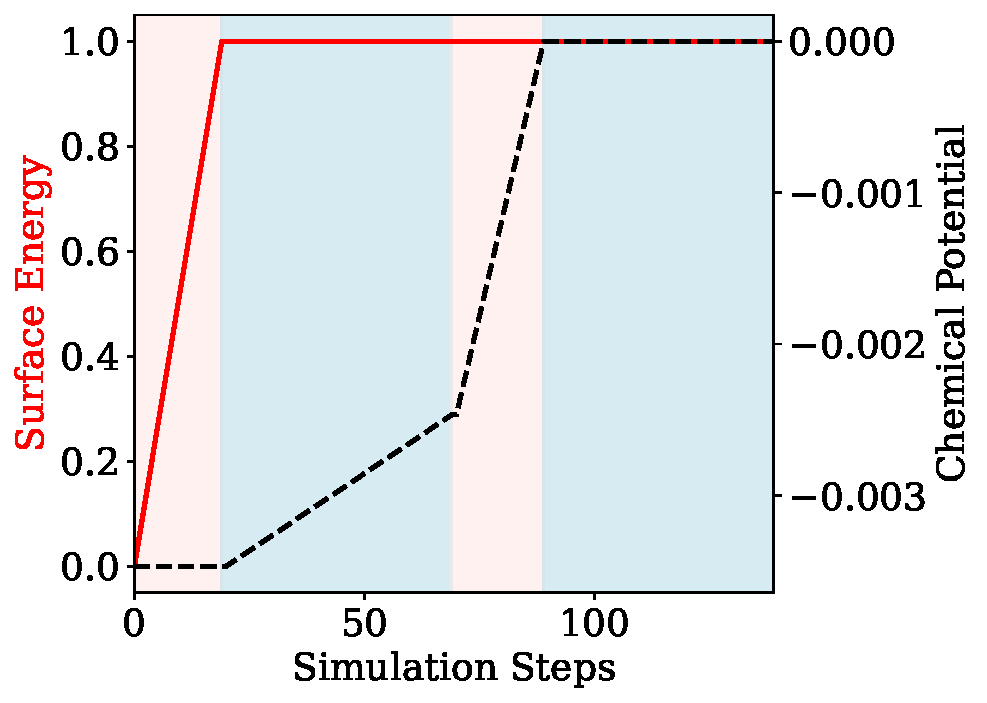
\includegraphics[width=0.49\textwidth]{../Images/SphereSimSteps}
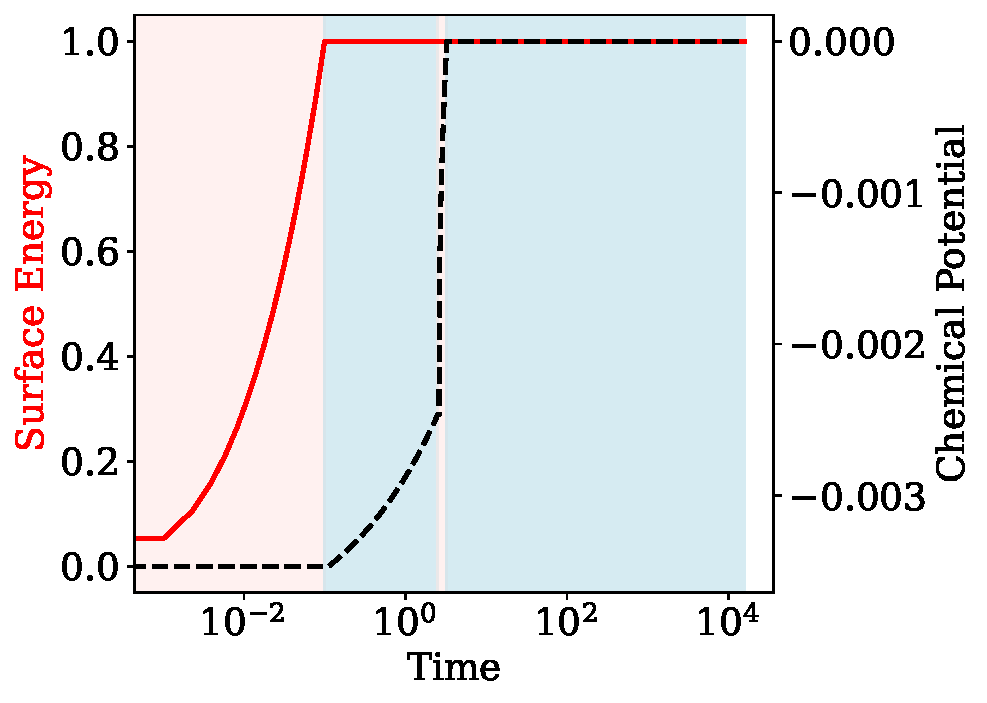
\includegraphics[width=0.49\textwidth]{../Images/SphereSimTime}
\caption{Example of ramping scheme for a free sphere where active ramping is illustrated with red shading and equilibration is demonstrated with blue regions over 1) simulation steps and 2) normalized simulation time. }
\label{FigRampingRegime}
\end{figure*}

Three codes are included pertaining to different geometries or boundary conditions. In order, 1) a free sphere 2) a free cube and 3) a cube fixed on the bottom. \\
{\fontfamily{qcr}\selectfont 
PoroelasticSphere.py \\
PoroelasticCubeFree.py \\
PoroelasticCube.py \\ \\ 
}
Lastly, there is a {\fontfamily{qcr}\selectfont PostProc.py} code that allows for plotting of the various parameters that are saved in txt files. For example, the displacement of a point on the boundary (0,0,1) for the sphere or (0,0,0.5) for the cubes can be tracked over the time evolution of the simulation. Fig. \ref{FigDispEvo} plots the displacement over time for a free sphere and free cube respectively, where the application of some amount of surface energy (constant, fluid-like assumption) leads to some contraction of the geometry, and a change in chemical potential from a negative starting value to $\hat{\mu} = 0$ leads to expansion of the geometry. 

\begin{figure*}[!htb]
\centering
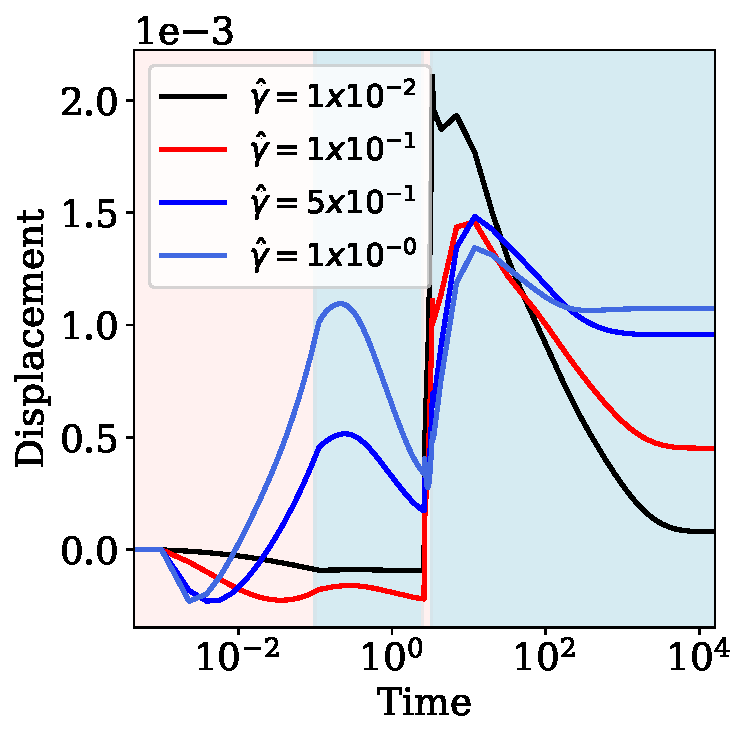
\includegraphics[width=0.4\textwidth]{../Images/SphereDispEvoGv}
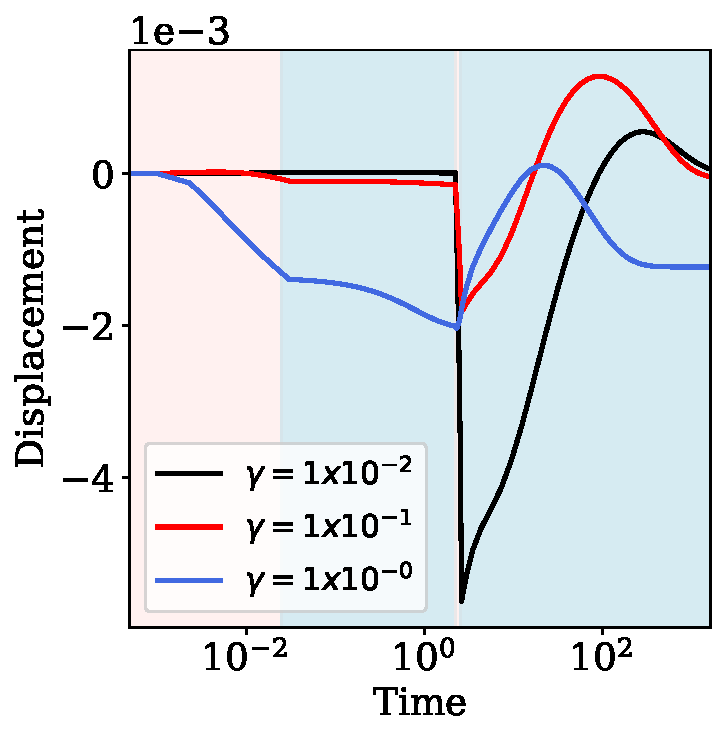
\includegraphics[width=0.39\textwidth]{../Images/CubeFreeDispEvoGv}
\caption{Displacement evolution of a A) point (0,0,1) on the boundary of a sphere and B) point (0,0,0.5) on the boundary cf the cube, where comparisons are made for different surface energy values. }
\label{FigDispEvo}
\end{figure*}
Since the ramping is largely a fictitious construct, we are more interested in the final equilibrium state. 

\newpage 

Fig. \ref{FigSphereChemEvo} demonstrates the chemical potential equilibrating for different values of surface energy. Note that this particular case uses quite large elements (check the gmsh files), and in the early stages oscillations in chemical potential occur over the first two surface elements. 

\begin{figure*}[!htb]
\centering
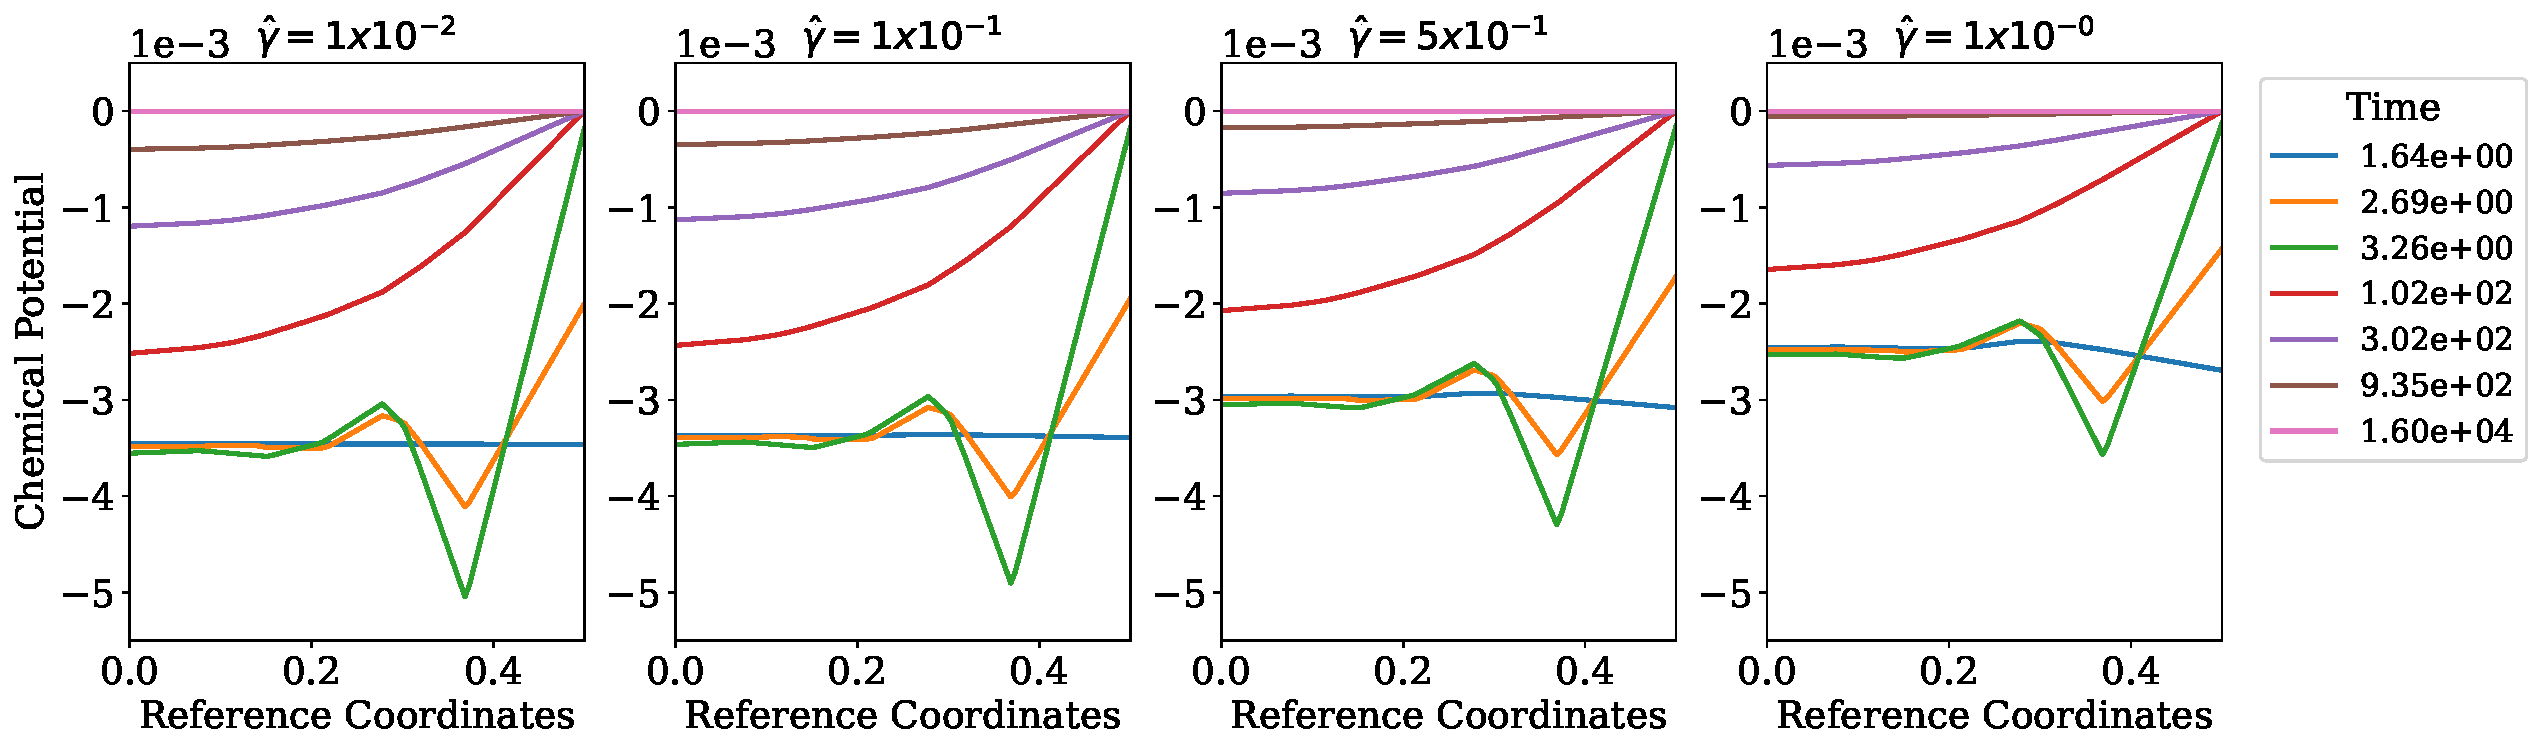
\includegraphics[width=\textwidth]{../Images/SphereChemEvoGv}
\caption{Different surface energy values from A) $1 \times 10^{-2}$ B) $1 \times 10^{-1}$ C) $5 \times 10^{-1}$ and D) $1 \times 10^{0}$. }
\label{FigSphereChemEvo}
\end{figure*}

Screenshots of Fig. \ref{FigSphereChemEvo}D) for the case where $\hat{\gamma} = 1 \times 10^{0}$. Swelling of the sphere can be observed from the initial step to the final step. 

\begin{figure*}[!htb]
\centering
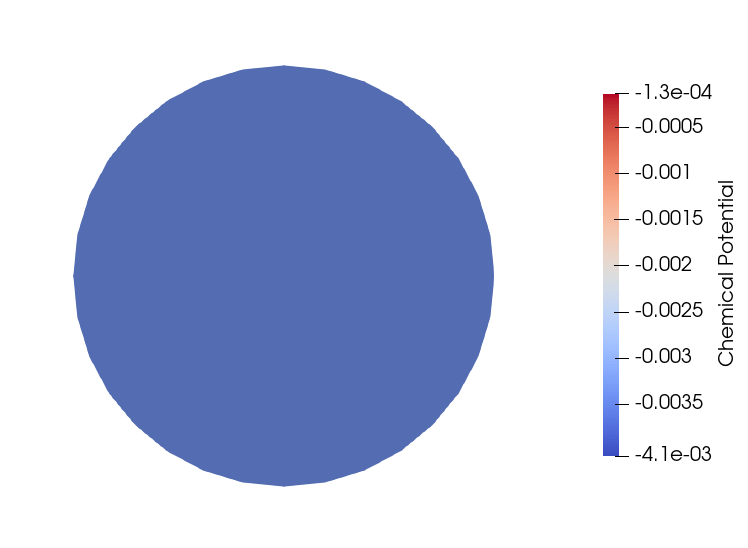
\includegraphics[width=0.24\textwidth]{../Results/Sphere/S_140_chi_3.0e-01_G_1e+00_l0_2.0e+00/Images/ChemicalPotential/ChemPot_000}
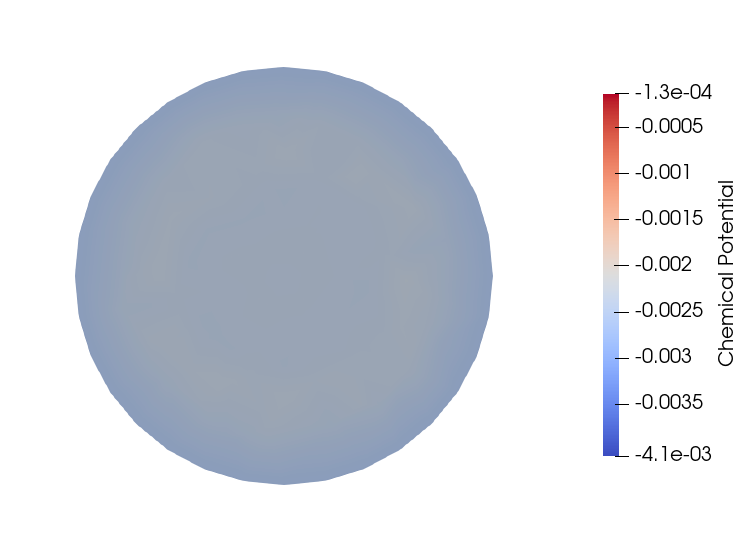
\includegraphics[width=0.24\textwidth]{../Results/Sphere/S_140_chi_3.0e-01_G_1e+00_l0_2.0e+00/Images/ChemicalPotential/ChemPot_059}
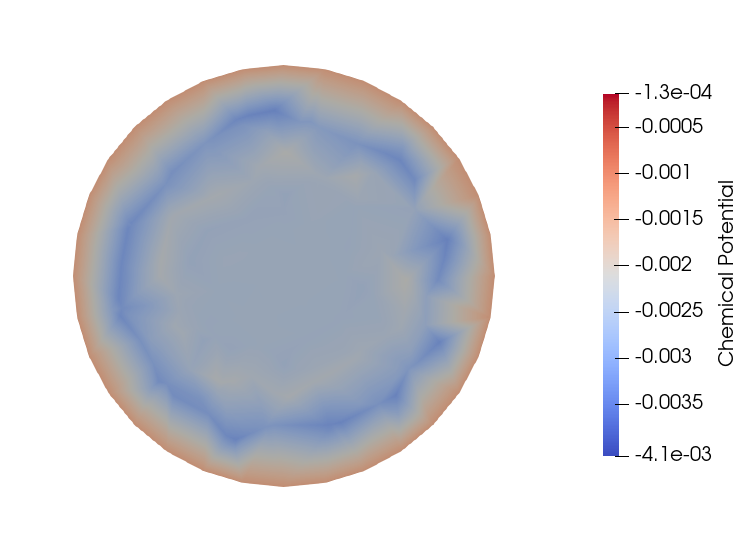
\includegraphics[width=0.24\textwidth]{../Results/Sphere/S_140_chi_3.0e-01_G_1e+00_l0_2.0e+00/Images/ChemicalPotential/ChemPot_079}
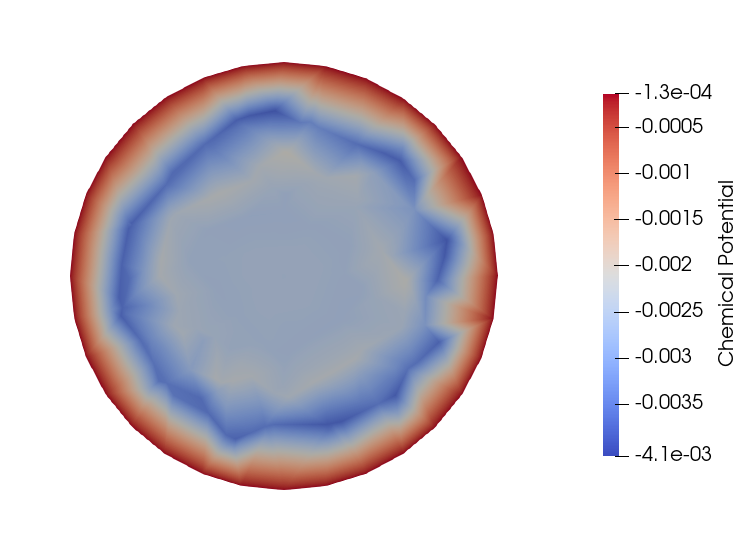
\includegraphics[width=0.24\textwidth]{../Results/Sphere/S_140_chi_3.0e-01_G_1e+00_l0_2.0e+00/Images/ChemicalPotential/ChemPot_089}
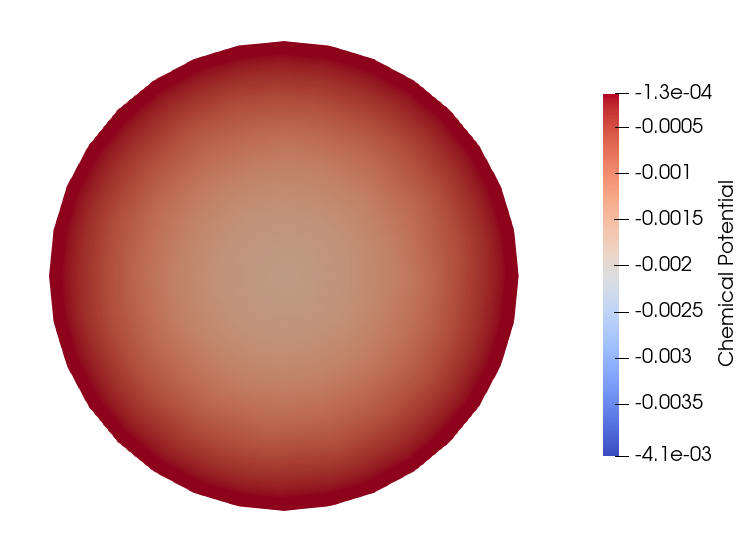
\includegraphics[width=0.24\textwidth]{../Results/Sphere/S_140_chi_3.0e-01_G_1e+00_l0_2.0e+00/Images/ChemicalPotential/ChemPot_099}
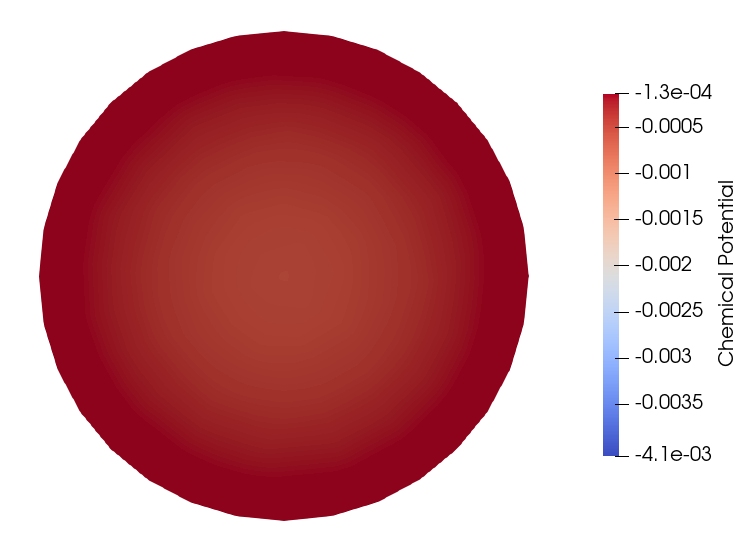
\includegraphics[width=0.24\textwidth]{../Results/Sphere/S_140_chi_3.0e-01_G_1e+00_l0_2.0e+00/Images/ChemicalPotential/ChemPot_103}
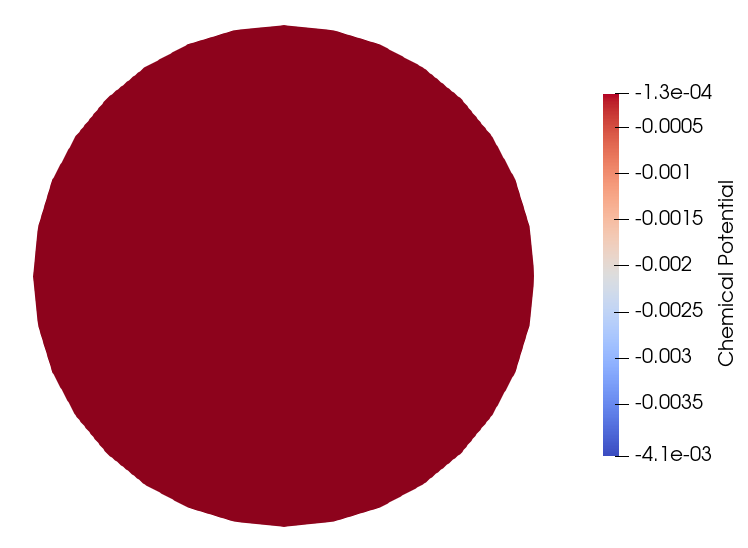
\includegraphics[width=0.24\textwidth]{../Results/Sphere/S_140_chi_3.0e-01_G_1e+00_l0_2.0e+00/Images/ChemicalPotential/ChemPot_109}
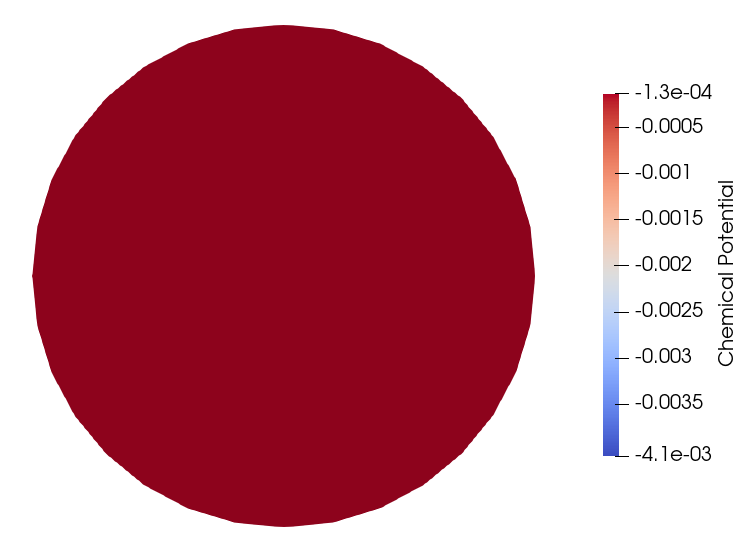
\includegraphics[width=0.24\textwidth]{../Results/Sphere/S_140_chi_3.0e-01_G_1e+00_l0_2.0e+00/Images/ChemicalPotential/ChemPot_139}
\caption{Change in chemical potential over time pertaining to the exact time steps from the prior figure in the current configuration.}
\label{FigSphereChemEvo}
\end{figure*}



\end{document}